\documentclass[10pt,twocolumn,letterpaper]{article}
\usepackage[review,applications]{wacv}
\usepackage[table]{xcolor}
\input{preamble}

\definecolor{wacvblue}{rgb}{0.21,0.49,0.74}
\usepackage[pagebackref,breaklinks,colorlinks,allcolors=wacvblue]{hyperref}
\def\wacvPaperID{2267} 
\def\confName{WACV}
\def\confYear{2027}

% Adjust float parameters to eliminate sparse empty spaces
\renewcommand{\topfraction}{0.95}
\renewcommand{\bottomfraction}{0.95}
\renewcommand{\textfraction}{0.05}
\renewcommand{\floatpagefraction}{0.85}
\setlength{\floatsep}{6pt plus 2pt minus 2pt}
\setlength{\textfloatsep}{8pt plus 2pt minus 2pt}
\setlength{\intextsep}{6pt plus 2pt minus 2pt}

\renewcommand{\thesection}{S\arabic{section}}
\renewcommand{\thetable}{S\arabic{table}}
\renewcommand{\thefigure}{S\arabic{figure}}
\renewcommand{\theequation}{S\arabic{equation}}
\setcounter{section}{0}
\setcounter{table}{0}
\setcounter{figure}{0}
\setcounter{equation}{0}

\title{Supplementary Material: Can Aesthetic Emotions Explain Individual Taste? \\Investigating an Interpretable Route to Personalized Image Aesthetics}
\author{Paper ID 2267}

\begin{document}
\maketitle

This document provides complete experimental protocols, reports the extended model and mediator analyses, and provides unit-level
faithfulness diagnostics tables supporting the main manuscript.
% ==================================================
\section{Experimental and Statistical Details}
\label{sec:supp_exp_stat}
% ===================================================

% -----------dataset detail----------------------
\subsection{Dataset Breakdown and First-Session Filtering}

XPASS-Vis dataset~\cite{hayashi2026xpassvis} contains 6,526 images, 129 participants,
and 87,836 user--image interactions across three visual domains (\cref{tab:domain_counts}). 
The released file encodes aesthetic scores as 0--6 and emotion responses as 0--4. The loader shifts the emotion items to 1--5; leaving the aesthetic score on its 0--6 file coding has no effect on SROCC or PLCC because both are invariant to a constant shift.

\begin{table}[h]
\centering
\caption{XPASS-Vis images and rating interactions per domain.}
\label{tab:domain_counts}
\begin{tabular}{lrr}
\toprule
Domain & Images & Interactions \\
\midrule
Artwork    & 2{,}345 & 31{,}543 \\
Fashion    & 2{,}082 & 28{,}154 \\
Landscape  & 2{,}099 & 28{,}139 \\
\midrule
Total      & 6{,}526 & 87{,}836 \\
\bottomrule
\end{tabular}
\end{table}

Approximately 5\% of ratings (4,509 of 87,836) are repeat evaluations where a participant rated the same image in separate sessions. 
We use only the first-occurring rating in the
released file and reserve the second occurrence exclusively for test-retest reliability (Tab.~1). Here,
``first'' means first in the occurrence order preserved by the released file;
reversing the pair would not change the symmetric test--retest correlation. This leaving 83,327 ratings for all experiments.
The filtering rule is deterministic and is applied before any split-specific data are built.
% ------------------------------------
\subsection{Leak-Free Split and Model Selection}
The 129 participants are partitioned into 10 fixed groups. Each of five folds
uses seven groups for training, one for validation, and two for testing; every
participant is a test user in exactly one fold. 
Participants and their rated images never  The exact user counts are shown
in \cref{tab:fold_counts}. Train, validation, and test participants are
disjoint, and images associated with these groups do not cross split
boundaries. Stage~1 and the population model are fitted only on training-group
images.

\begin{table}[t]
\centering
\caption{Fixed participant split used in every experiment.}
\label{tab:fold_counts}
\begin{tabular}{crrrr}
\toprule
Fold & Train & Validation & Test & Stage-1 train images \\
\midrule
0 & 97 &  6 & 26 & 4{,}561 \\
1 & 95 & 12 & 22 & 4{,}564 \\
2 & 92 & 14 & 23 & 4{,}563 \\
3 & 83 & 16 & 30 & 4{,}561 \\
4 & 84 & 17 & 28 & 4{,}582 \\
\bottomrule
\end{tabular}
\end{table}

Within each user and domain, a deterministic seed (texttt{RandomState(42 + user\_id)})
first holds out 50 evaluation images. Support sets of $N\in\{10,25,50,100\}$ are then taken from the remainder, so every rating budget is evaluated on the same images. A candidate personal-head hyperparameter is fitted separately on each validation user's support set and scored by SROCC on that user's disjoint 50-image validation evaluation set.
Scores are averaged across validation-user units; one candidate is frozen for the fold--domain--condition--budget combination and applied to all test users.
Shared components are selected by validation-group image-level MSE.

Ridge uses 17 penalties from $10^{-2}$ to $10^{6}$
($\operatorname{logspace}(-2,6,17)$). MLPs have one 128-unit ReLU hidden layer,
Adam optimization, MSE loss, no weight decay, and a fixed 500-epoch budget.
Their learning rate is selected from
$\{10^{-4},3\!\times\!10^{-4},\ldots,3,10\}$. Early stopping is disabled:
at $N=10$, an internal hold-out would contain only one or two observations.

% -------------------------------------------------
\subsection{Inference and Holm--Bonferroni Families}

SROCC and PLCC are computed on held-out images for each user--domain unit.
Domain-specific comparisons use 129 paired participants and two-sided
Wilcoxon signed-rank tests. For an Average column, the three domains from one
participant are correlated; therefore the mean uncertainty, confidence
interval, and two-sided test use 10,000 participant-cluster bootstrap samples
(seed 0), resampling 129 participants and retaining all three domains as a
block. Empirical tail probabilities are estimated from those 10,000 samples;
a zero tail count is not interpreted as an exact zero and is reported as
$p<.001$. Weight-alignment tests are one-sided because the tested alternative
is directional and positive.

Holm--Bonferroni correction is applied separately within each family in
\cref{tab:holm_families}. SROCC and PLCC are always separate families, and an
Average family is never combined with a domain-specific family. Tables not
listed there are descriptive and carry no significance markers.
The family definitions were fixed before the final correction audit was run;
they were not registered in advance.

\begin{table*}[t]
\centering
\caption{Multiple-comparison families used in the final audit. ``Domain'' comprises
Artwork, Fashion, Landscape, and a separate clustered Average family.}
\label{tab:holm_families}
\small
\setlength{\tabcolsep}{5pt}
\begin{tabular}{p{2.2cm}p{2.6cm}p{6.3cm}p{2.3cm}r}
\toprule
Result block & Family defined by & Reference contrast(s) & Test & Size \\
\midrule
Main Table 1 & domain $\times$ metric & Hybrid vs Population, Direct, Random, PCA & paired / cluster & 4 \\
Anchor Table 2 & Average $\times$ metric & Hybrid vs four mediators, both anchor settings & cluster & 8 \\
Backbone Table S2 & domain $\times$ metric & Hybrid vs Population across five backbones & paired / cluster & 5 \\
Efficiency Fig.~4 & domain $\times$ metric & Hybrid and Direct vs Population at four budgets & paired / cluster & 8 \\
Faithfulness tables & domain $\times$ metric & formula (6), anchored ablation (3), image (4) & paired / cluster & 13 \\
Weight alignment Table 4 & domain $\times$ coefficient type & alignment greater than zero & one-sided / cluster & 1 \\
\bottomrule
\end{tabular}
\end{table*}

For traceability, the released statistics CSV also retains 24 exploratory
MLP contrasts and 12 exploratory distribution-target contrasts. Their tables
below are descriptive: these retained calculations do not create manuscript
significance markers or support inferential claims.

% --------reproducibility---------------
\subsection{Reproducibility and Released Artifacts}

BLAS operations are pinned to one thread before NumPy is imported. Random
projections, permutations, and initializations use fixed seeds; validation
ties within a relative tolerance of $10^{-9}$ are resolved by a deterministic
conservative rule. The released \texttt{uv.lock} is the executable reference
environment. The final audit used Python 3.13.5, NumPy 2.5.2, pandas 3.0.5,
SciPy 1.18.0, scikit-learn 1.9.0, and Matplotlib 3.11.1. Training runs were
produced on more than one platform; all reported values are retained
as per-unit outputs, and the locked environment regenerates the downstream
statistics and presentation artifacts from those outputs.

The emotion, PCA, and identity ridge pipelines are deterministic for a fixed
split and support set. Seed averaging therefore affects the stochastic Random
and Shuffled controls and the MLP conditions, but does not create three
independent versions of each deterministic ridge result. Each participant has
one deterministic support-set draw, so the reported uncertainty is conditional
on that draw; it does not quantify variation under new support images. Shared
fold-level components are likewise treated as fixed by the reported
participant-level inference.

The release includes the fixed split files and eleven compact audit-facing
CSV files:
\texttt{raw\_all\_final.csv} (seed-level model results),
\texttt{formula\_units\_final.csv} and
\texttt{formula\_images\_final.csv} (formula and image-level diagnostics),
\texttt{stage1\_accuracy.csv},
\texttt{statistics/holm\_corrected.csv}. The set also contains
\texttt{upper\_bound\_units\_final.csv},
\texttt{emotion\_importance\_units\_final.csv},
\texttt{mlp\_architecture\_units\_final.csv},
\texttt{reference\_bounds\_final.csv}, and
\texttt{regularizer\_units\_final.csv}, together with the 387-row
\texttt{test\_retest\_units.csv} used for the within-unit reference.
Three small source manifests record
the contributing files and their SHA-256 hashes.
The licensed raw ratings and large extracted features are not redistributed;
their expected schemas and extraction commands are documented in the code
package included with this supplementary material.

The frozen per-unit outputs are the numerical source of the release. The locked
environment regenerates downstream statistics, tables, and figures, and
\texttt{reproduce.py} compares the regenerated Holm table row-for-row with the
frozen audit.
Code, reproduction scripts, and frozen databases are available at \url{https://anonymous.4open.science/r/piaa-emotion-mediated-anonymous-DF01/}.



\subsection{Reference Quantities}

The ground-truth-emotion (GT) reference replaces Stage~1 predictions with each
user's reported emotions and fits an unanchored ridge head. Unlike the compared
model rows, its penalty is selected per user by RidgeCV on that user's support
set. It is therefore an optimistic diagnostic of perfect emotion observation
rather than a deployable condition trained under the matched selection rule.

The test--retest reference can be summarized either by pooling all repeated
pairs or by first computing a correlation within each user--domain unit. The
former is the .684 SROCC reported as a dataset-level reference; the latter is
on the same within-user scale as the model scores (Table~\ref{tab:retest_units}).
Because each unit contains a median of only 12 repeated images (range 5--12),
the within-unit correlations are themselves noisy and are provided as a scale
reference rather than a model comparison.

\begin{table}[!htbp]
\centering
\begin{threeparttable}
\caption{Test--retest correlation under two aggregation rules.}
\label{tab:retest_units}
\scriptsize
\setlength{\tabcolsep}{2pt}
\begin{tabular}{llcccc}
\toprule
Metric & Aggregation & Art & Fash. & Land. & Avg. \\
\midrule
\multirow{2}{*}{SROCC}
 & Pooled pairs & .672 & .688 & .695 & .684 \\
 & Within unit  & .577 & .593 & .584 & .585 \\
\addlinespace
\multirow{2}{*}{PLCC}
 & Pooled pairs & .686 & .691 & .703 & .693 \\
 & Within unit  & .589 & .595 & .607 & .597 \\
\bottomrule
\end{tabular}
\begin{tablenotes}[flushleft]\footnotesize
\item Pooled rows contain 4,509 repeated pairs. Within-unit rows average 387
user--domain correlations; the participant-cluster 95\% interval for Average
SROCC is [.550, .617].
\end{tablenotes}
\end{threeparttable}
\end{table}

% ========================2===========================
\section{Extended Model Architecture and Performance}
\label{sec:supp_arch_perf}
% ==============================================
\subsection{Visual Backbone Robustness}
\cref{tab:backbone} presents the full breakdown of Population, Direct, and Hybrid models across all five evaluated backbones and three image domains.
%----- Table S2: Backbone
\begin{table*}[tbp]
\centering
\footnotesize
\setlength{\tabcolsep}{4.5pt}
\caption{Population, Direct, and Hybrid ridge models across visual backbones
and domains.}
\label{tab:backbone}
\begin{threeparttable}
    \begin{tabular}{ll cc cc cc cc}
\toprule
\multirow{2}{*}{Backbone} & \multirow{2}{*}{Model} & \multicolumn{2}{c}{Artwork} & \multicolumn{2}{c}{Fashion} & \multicolumn{2}{c}{Landscape} & \multicolumn{2}{c}{Average} \\
\cmidrule(lr){3-4}\cmidrule(lr){5-6}\cmidrule(lr){7-8}\cmidrule(lr){9-10}
 & & SROCC & PLCC & SROCC & PLCC & SROCC & PLCC & SROCC & PLCC \\
\midrule
\multirow{3}{*}{CLIP frozen} & Population & $.465_{\pm .017}$ & $.474_{\pm .016}$ & $.326_{\pm .013}$ & $.347_{\pm .013}$ & $.457_{\pm .015}$ & $.459_{\pm .014}$ & $.416_{\pm .011}$ & $.427_{\pm .011}$ \\
& Direct & $\bm{.524_{\pm .014}}$ & $\bm{.533_{\pm .014}}$ & $\bm{.365_{\pm .013}}$ & $\bm{.382_{\pm .013}}$ & $.478_{\pm .015}$ & $\bm{.489_{\pm .014}}$ & $\bm{.456_{\pm .011}}$ & $\bm{.468_{\pm .010}}$ \\
& Hybrid & $.486_{\pm .017}^{\dagger}$ & $.493_{\pm .016}^{\dagger}$ & $.338_{\pm .014}$ & $.356_{\pm .013}^{\dagger}$ & $\bm{.481_{\pm .014}}^{\dagger}$ & $.486_{\pm .014}^{\dagger}$ & $.435_{\pm .011}^{\dagger}$ & $.445_{\pm .011}^{\dagger}$ \\
\addlinespace
\multirow{3}{*}{CLIP-ft (score)} & Population & $.470_{\pm .017}$ & $.477_{\pm .016}$ & $.332_{\pm .013}$ & $.347_{\pm .013}$ & $.452_{\pm .014}$ & $.455_{\pm .014}$ & $.418_{\pm .011}$ & $.426_{\pm .010}$ \\
& Direct & $\bm{.539_{\pm .013}}$ & $\bm{.542_{\pm .013}}$ & $\bm{.355_{\pm .013}}$ & $\bm{.375_{\pm .013}}$ & $\bm{.482_{\pm .015}}$ & $\bm{.487_{\pm .014}}$ & $\bm{.459_{\pm .010}}$ & $\bm{.468_{\pm .010}}$ \\
& Hybrid & $.488_{\pm .016}^{\dagger}$ & $.493_{\pm .016}$ & $.340_{\pm .013}$ & $.353_{\pm .013}$ & $.472_{\pm .014}^{\dagger}$ & $.477_{\pm .014}^{\dagger}$ & $.434_{\pm .011}^{\dagger}$ & $.441_{\pm .010}^{\dagger}$ \\
\addlinespace
\multirow{3}{*}{CLIP-ft (emotion)} & Population & $.468_{\pm .016}$ & $.473_{\pm .016}$ & $.315_{\pm .014}$ & $.329_{\pm .013}$ & $.435_{\pm .015}$ & $.438_{\pm .014}$ & $.406_{\pm .011}$ & $.413_{\pm .010}$ \\
& Direct & $\bm{.525_{\pm .013}}$ & $\bm{.531_{\pm .013}}$ & $\bm{.349_{\pm .015}}$ & $\bm{.362_{\pm .014}}$ & $\bm{.473_{\pm .015}}$ & $\bm{.479_{\pm .015}}$ & $\bm{.449_{\pm .011}}$ & $\bm{.457_{\pm .011}}$ \\
& Hybrid & $.486_{\pm .015}^{\dagger}$ & $.492_{\pm .015}^{\dagger}$ & $.328_{\pm .015}$ & $.341_{\pm .015}$ & $.456_{\pm .015}^{\dagger}$ & $.463_{\pm .015}^{\dagger}$ & $.423_{\pm .011}^{\dagger}$ & $.432_{\pm .011}^{\dagger}$ \\
\addlinespace
\multirow{3}{*}{Qwen3-VL 4B} & Population & $.476_{\pm .017}$ & $.486_{\pm .016}$ & $.363_{\pm .013}$ & $.374_{\pm .013}$ & $.469_{\pm .014}$ & $.472_{\pm .014}$ & $.436_{\pm .011}$ & $.444_{\pm .011}$ \\
& Direct & $\bm{.532_{\pm .013}}$ & $\bm{.539_{\pm .013}}$ & $\bm{.382_{\pm .014}}$ & $\bm{.394_{\pm .013}}$ & $\bm{.496_{\pm .014}}$ & $\bm{.501_{\pm .014}}$ & $\bm{.470_{\pm .011}}$ & $\bm{.478_{\pm .010}}$ \\
& Hybrid & $.488_{\pm .016}$ & $.495_{\pm .016}$ & $.365_{\pm .015}$ & $.377_{\pm .014}$ & $.492_{\pm .014}^{\dagger}$ & $.499_{\pm .014}^{\dagger}$ & $.448_{\pm .012}^{\dagger}$ & $.457_{\pm .011}^{\dagger}$ \\
\addlinespace
\multirow{3}{*}{Qwen3-VL 8B} & Population & $.477_{\pm .017}$ & $.487_{\pm .017}$ & $.372_{\pm .013}$ & $.384_{\pm .013}$ & $.469_{\pm .015}$ & $.475_{\pm .014}$ & $.439_{\pm .011}$ & $.449_{\pm .011}$ \\
& Direct & $\bm{.534_{\pm .014}}$ & $\bm{.542_{\pm .014}}$ & $\bm{.398_{\pm .013}}$ & $\bm{.412_{\pm .013}}$ & $\bm{.501_{\pm .015}}$ & $\bm{.510_{\pm .015}}$ & $\bm{.478_{\pm .011}}$ & $\bm{.488_{\pm .010}}$ \\
& Hybrid & $.496_{\pm .016}^{\dagger}$ & $.504_{\pm .016}$ & $.386_{\pm .014}$ & $.398_{\pm .013}^{\dagger}$ & $.496_{\pm .015}^{\dagger}$ & $.504_{\pm .015}^{\dagger}$ & $.459_{\pm .011}^{\dagger}$ & $.469_{\pm .011}^{\dagger}$ \\
\bottomrule
\end{tabular}
    \begin{tablenotes}[flushleft]\footnotesize
    \item Values are mean $\pm$ SEM. Domain columns use 129 participants; Average uses the participant-cluster bootstrap over the same 129 participants.
    \item $\dagger$ marks Hybrid above Population after Holm correction within the corresponding domain--metric family across five backbones. Direct is descriptive and is not included in that family. The best predictive value in each cell block is shown in \textbf{bold}.
    \end{tablenotes}
\end{threeparttable}
\end{table*}

\begin{table}[!htbp]
\centering
\begin{threeparttable}
\caption{Same-width Hybrid and PCA mediators across backbones at $N=100$.
Values are Average SROCC.}
\label{tab:mediator_backbone}
\small
\begin{tabular}{lccc}
    \toprule
    Backbone & Hybrid & PCA & Hybrid--PCA (95\% CI) \\
    \midrule
    \multicolumn{4}{l}{\textit{Anchored}}\\
    \addlinespace[2pt]
    CLIP frozen       & $.435$ & $.445$ & $-.010$ $[-.018,-.003]$ \\
    CLIP-ft (score)   & $.434$ & $.446$ & $-.013$ $[-.021,-.005]$ \\
    CLIP-ft (emotion) & $.423$ & $.441$ & $-.018$ $[-.025,-.011]$ \\
    Qwen3-VL 4B       & $.448$ & $.454$ & $-.006$ $[-.014,+.002]$ \\
    Qwen3-VL 8B       & $.459$ & $.458$ & $+.001$ $[-.006,+.008]$ \\
    \midrule
    \multicolumn{4}{l}{\textit{Unanchored}}\\
    \addlinespace[2pt]
    CLIP frozen       & $.419$ & $.377$ & $+.041$ $[+.029,+.053]$ \\
    CLIP-ft (score)   & $.427$ & $.425$ & $+.002$ $[-.007,+.011]$ \\
    CLIP-ft (emotion) & $.419$ & $.421$ & $-.002$ $[-.011,+.006]$ \\
    Qwen3-VL 4B       & $.436$ & $.362$ & $+.073$ $[+.061,+.086]$ \\
    Qwen3-VL 8B       & $.446$ & $.382$ & $+.063$ $[+.051,+.075]$ \\
    \bottomrule
\end{tabular}
\begin{tablenotes}[flushleft]\footnotesize
    \item Differences and intervals are participant-cluster bootstrap estimates
    over 129 participants. This descriptive scope analysis adds no Holm contrasts.
    On the primary Qwen3-VL 8B backbone, anchored Hybrid and PCA differ by only
    $+.001$ (95\% CI $[-.006,.008]$); this near-equality does not extend to the
    three CLIP variants. Without anchoring, Hybrid is higher on three backbones,
    while the intervals for the two CLIP-ft variants include zero.
\end{tablenotes}
\end{threeparttable}
\end{table}
% ---------------------------------------
\subsection{Linear and Nonlinear Heads}
\label{sec:supp_joint}
%  --------MLP -----------
The sequential MLP first fits a shared emotion extractor and freezes it before
fitting a personal MLP. In the joint variant, the shared extractor is trained
with
\begin{equation}
\mathcal{L}=\operatorname{MSE}(\hat y)+
\lambda\operatorname{MSE}(\hat{\mathbf e}),
\qquad \lambda\in\{0.1,1,10\},
\end{equation}
where the emotion loss is averaged over seven concepts. Task gradients pass
through the semantic layer, following the joint concept-bottleneck setup of
Koh et al.~\cite{pmlr-v119-koh20a}. Joint training is restricted to the shared
stage; it does not fine-tune a high-capacity extractor separately for each
user.
% ---------------MLP baseline---------------
\begin{table*}[!tbp]
\centering
\begin{threeparttable}
\caption{Ridge and sequential MLP heads for each mediator. Qwen3-VL 8B,
population-anchored, $N=100$.}
\label{tab:mlp_baseline}
\footnotesize
    \begin{tabular}{ll cc cc cc cc}
\toprule
\multirow{2}{*}{Mediator} & \multirow{2}{*}{Head} & \multicolumn{2}{c}{Artwork} & \multicolumn{2}{c}{Fashion} & \multicolumn{2}{c}{Landscape} & \multicolumn{2}{c}{Average} \\
\cmidrule(lr){3-4}\cmidrule(lr){5-6}\cmidrule(lr){7-8}\cmidrule(lr){9-10}
& & SROCC & PLCC & SROCC & PLCC & SROCC & PLCC & SROCC & PLCC \\
\midrule
\multirow{2}{*}{Population} & Ridge & $.477_{\pm .017}$ & $.487_{\pm .017}$ & $.372_{\pm .013}$ & $.384_{\pm .013}$ & $.469_{\pm .015}$ & $.475_{\pm .014}$ & $.439_{\pm .011}$ & $.449_{\pm .011}$ \\
 & MLP & $.427_{\pm .016}$ & $.438_{\pm .016}$ & $.303_{\pm .011}$ & $.316_{\pm .012}$ & $.401_{\pm .013}$ & $.406_{\pm .013}$ & $.377_{\pm .010}$ & $.386_{\pm .010}$ \\
\addlinespace
\multirow{2}{*}{Direct} & Ridge & $.534_{\pm .014}$ & $.542_{\pm .014}$ & $.398_{\pm .013}$ & $.412_{\pm .013}$ & $.501_{\pm .015}$ & $.510_{\pm .015}$ & $.478_{\pm .011}$ & $.488_{\pm .010}$ \\
 & MLP & $.356_{\pm .014}$ & $.354_{\pm .014}$ & $.234_{\pm .012}$ & $.238_{\pm .012}$ & $.336_{\pm .015}$ & $.339_{\pm .015}$ & $.309_{\pm .010}$ & $.310_{\pm .010}$ \\
\addlinespace
\multirow{2}{*}{Random} & Ridge & $.495_{\pm .015}$ & $.504_{\pm .015}$ & $.373_{\pm .013}$ & $.384_{\pm .012}$ & $.473_{\pm .014}$ & $.480_{\pm .014}$ & $.447_{\pm .010}$ & $.456_{\pm .010}$ \\
 & MLP & $.479_{\pm .013}$ & $.484_{\pm .014}$ & $.328_{\pm .012}$ & $.339_{\pm .012}$ & $.431_{\pm .014}$ & $.431_{\pm .014}$ & $.412_{\pm .010}$ & $.418_{\pm .010}$ \\
\addlinespace
\multirow{2}{*}{PCA} & Ridge & $.510_{\pm .015}$ & $.519_{\pm .015}$ & $.377_{\pm .014}$ & $.388_{\pm .013}$ & $.487_{\pm .015}$ & $.495_{\pm .015}$ & $.458_{\pm .011}$ & $.467_{\pm .011}$ \\
 & MLP & $.495_{\pm .015}$ & $.504_{\pm .015}$ & $.350_{\pm .013}$ & $.359_{\pm .013}$ & $.466_{\pm .016}$ & $.469_{\pm .016}$ & $.437_{\pm .011}$ & $.444_{\pm .011}$ \\
\addlinespace
\multirow{2}{*}{Hybrid (ours)} & Ridge & $.496_{\pm .016}$ & $.504_{\pm .016}$ & $.386_{\pm .014}$ & $.398_{\pm .013}$ & $.496_{\pm .015}$ & $.504_{\pm .015}$ & $.459_{\pm .011}$ & $.469_{\pm .011}$ \\
 & MLP & $.459_{\pm .015}$ & $.468_{\pm .016}$ & $.315_{\pm .013}$ & $.325_{\pm .012}$ & $.437_{\pm .015}$ & $.441_{\pm .014}$ & $.404_{\pm .011}$ & $.411_{\pm .010}$ \\
\bottomrule
\end{tabular}

% Descriptive table: no significance markers.
% Qwen3-VL 8B, population-anchored, N=100; seeds averaged within units.

\begin{tablenotes}[flushleft]\footnotesize
\item Values are mean $\pm$ SEM after averaging seeds within units. Average
SEM uses the participant-cluster bootstrap. This table is descriptive and
contains no hypothesis tests.
\end{tablenotes}
\end{threeparttable}
\end{table*}

\begin{table*}[!tbp]
\centering
\begin{threeparttable}
\caption{Sequential and joint MLP training for the Hybrid mediator. Qwen3-VL
8B, population-anchored, $N=100$.}
\label{tab:mlp}
\footnotesize
    \begin{tabular}{@{}l cc cc cc cc@{}}
\toprule
\multirow{2}{*}{Stage-1 $\to$ Stage-2} & \multicolumn{2}{c}{Artwork} & \multicolumn{2}{c}{Fashion} & \multicolumn{2}{c}{Landscape} & \multicolumn{2}{c}{Average} \\
\cmidrule(lr){2-3}\cmidrule(lr){4-5}\cmidrule(lr){6-7}\cmidrule(lr){8-9}
& SROCC & PLCC & SROCC & PLCC & SROCC & PLCC & SROCC & PLCC \\
\midrule
Ridge $\to$ Ridge (main) & $\bm{.496_{\pm .016}}$ & $\bm{.504_{\pm .016}}$ & $\bm{.386_{\pm .014}}$ & $\bm{.398_{\pm .013}}$ & $\bm{.496_{\pm .015}}$ & $\bm{.504_{\pm .015}}$ & $\bm{.459_{\pm .011}}$ & $\bm{.469_{\pm .011}}$ \\
\addlinespace
MLP $\to$ MLP, joint $\lambda=0.1$ & $.430_{\pm .016}$ & $.437_{\pm .016}$ & $.278_{\pm .012}$ & $.289_{\pm .012}$ & $.392_{\pm .015}$ & $.395_{\pm .015}$ & $.367_{\pm .010}$ & $.374_{\pm .010}$ \\
MLP $\to$ MLP, joint $\lambda=1$ & $.450_{\pm .015}$ & $.456_{\pm .016}$ & $.301_{\pm .012}$ & $.315_{\pm .012}$ & $.413_{\pm .015}$ & $.415_{\pm .014}$ & $.388_{\pm .011}$ & $.395_{\pm .010}$ \\
MLP $\to$ MLP, joint $\lambda=10$ & $.460_{\pm .015}$ & $.467_{\pm .015}$ & $.310_{\pm .013}$ & $.323_{\pm .012}$ & $.436_{\pm .015}$ & $.439_{\pm .014}$ & $.402_{\pm .011}$ & $.410_{\pm .011}$ \\
\addlinespace
MLP $\to$ MLP, sequential & $.459_{\pm .015}$ & $.468_{\pm .016}$ & $.315_{\pm .013}$ & $.325_{\pm .012}$ & $.437_{\pm .015}$ & $.441_{\pm .014}$ & $.404_{\pm .011}$ & $.411_{\pm .010}$ \\
\bottomrule
\end{tabular}

% Descriptive table: no significance markers.
% Average SEM uses a 129-participant cluster bootstrap.

\begin{tablenotes}[flushleft]\footnotesize
    \item Values are mean $\pm$ SEM after averaging seeds within units. Average SEM uses the participant-cluster bootstrap. The evaluated MLP variants have lower mean SROCC and PLCC than Ridge $\to$ Ridge in every domain. The table is descriptive and contains no hypothesis tests.
\end{tablenotes}
\end{threeparttable}
\end{table*}

 % -------------linear rgressor ablation-----------
\subsection{Choice of Regularizer for Personal Heads}
\cref{tab:regulariser} compares Ridge ($\ell_2$), Lasso ($\ell_1$), and Elastic Net penalties. The 7-dimensional emotion bottleneck is robust across regularizers, whereas raw features suffer severe drops under sparsity penalties.

\begin{table*}[!tbp]
\centering
\begin{threeparttable}
\caption{Descriptive regularizer sensitivity for the personal head. Frozen
CLIP, unanchored models, $N=100$, and three seeds.}
\label{tab:regularizer}
\footnotesize
\setlength{\tabcolsep}{4pt}
    \begin{tabular}{@{}l cc cc cc@{}}
        \toprule
        \multirow{2}{*}{Head} & \multicolumn{2}{c}{Population} & \multicolumn{2}{c}{Direct} & \multicolumn{2}{c}{Hybrid} \\
        \cmidrule(lr){2-3}\cmidrule(lr){4-5}\cmidrule(lr){6-7}
        & SROCC & PLCC & SROCC & PLCC & SROCC & PLCC \\
        \midrule
        Ridge       & $.416_{\pm .011}$ & $.427_{\pm .011}$ & $.400_{\pm .012}$ & $.410_{\pm .012}$ & $.419_{\pm .011}$ & $.429_{\pm .011}$ \\
        Lasso       & $.412_{\pm .011}$ & $.422_{\pm .010}$ & $.330_{\pm .012}$ & $.340_{\pm .012}$ & $.417_{\pm .011}$ & $.427_{\pm .011}$ \\
        Elastic net & $.412_{\pm .011}$ & $.422_{\pm .010}$ & $.344_{\pm .012}$ & $.354_{\pm .012}$ & $.419_{\pm .011}$ & $.428_{\pm .011}$ \\
        \bottomrule
    \end{tabular}
\begin{tablenotes}[flushleft]\footnotesize
    \item Values are mean $\pm$ SEM after averaging the three seeds within each user--domain unit. SEM uses the participant-cluster bootstrap over 129 participants. This table is descriptive and has no significance markers.
    \item Sparse penalties produced a constant prediction in two Lasso--Hybrid units and one Elastic-Net--Hybrid unit, so their correlations are undefined and excluded from the corresponding mean and bootstrap (valid $n=385$ and $386$, respectively). Every other cell contains all 387 units.
    \item All heads were rerun together under the current split, support-set, and validation-selection protocol. Hybrid varies by at most .002 SROCC across the three regularizers, whereas sparse penalties reduce Direct by .055--.070. This supports Ridge as the common head used in the primary experiments.
\end{tablenotes}
\end{threeparttable}
\end{table*}

% ---efficientcy graph detail
\subsection{Detailed Rating-Budget Results}
\cref{tab:efficiency_full} provides the complete numerical values across sample sizes $N \in \{10, 25, 50, 100\}$ plotted in Fig. ~2 of the main manuscript.

\begin{table*}[!tbp]
\centering
\begin{threeparttable}
\caption{Population, Direct, and Hybrid performance across personal-rating
budgets with Qwen3-VL 8B and the population anchor.}
\label{tab:efficiency_full}
\fontsize{6.1}{7.2}\selectfont
\setlength{\tabcolsep}{1.2pt}
    \begin{tabular}{ll cc cc cc cc}
\toprule
\multirow{2}{*}{$N$} & \multirow{2}{*}{\textbf{Model}} 
  & \multicolumn{2}{c}{\textbf{Artwork}} 
  & \multicolumn{2}{c}{\textbf{Fashion}} 
  & \multicolumn{2}{c}{\textbf{Landscape}} 
  & \multicolumn{2}{c}{\textbf{Average}} \\
\cmidrule(lr){3-4} \cmidrule(lr){5-6} \cmidrule(lr){7-8} \cmidrule(lr){9-10}
  & & \textbf{SROCC} & \textbf{PLCC} 
    & \textbf{SROCC} & \textbf{PLCC} 
    & \textbf{SROCC} & \textbf{PLCC} 
    & \textbf{SROCC} & \textbf{PLCC} \\
\midrule
\multicolumn{2}{l}{\textit{Population}} 
  & $.477_{\pm .017}$ & $.487_{\pm .017}$ 
  & $.372_{\pm .013}$ & $.384_{\pm .013}$ 
  & $.469_{\pm .015}$ & $.475_{\pm .014}$ 
  & $.439_{\pm .009}$ & $.449_{\pm .009}$ \\
\addlinespace
10 & Direct & $.486_{_{\pm .016}}$ 
        & $.498_{_{\pm .016}}$ & $.368_{_{\pm .013}}$ 
        & $.381_{_{\pm .012}}$ & $.458_{_{\pm .015}}$ 
        & $.464_{_{\pm .015}}$ & $.437_{_{\pm .011}}$ 
        & $.448_{_{\pm .011}}$ \\
    & Hybrid & $.481_{\pm .017}$ & $.490_{\pm .016}$ 
        & $.347_{\pm .015}$ & $.360_{\pm .015}$ 
        & $.472_{\pm .015}$ & $.479_{\pm .015}$ 
        & $.433_{\pm .010}$ & $.443_{\pm .009}$ \\
\addlinespace
25 & Direct & $.494_{_{\pm .016}}$ & $.504_{_{\pm .016}}$ 
        & $.376_{_{\pm .013}}$ & $.389_{_{\pm .013}}$ 
        & $.481_{_{\pm .014}}$ & $.489_{_{\pm .014}}$ & $.450_{_{\pm .011}}$ & $.460_{_{\pm .011}}$ \\
   & Hybrid & $.478_{_{\pm .017}}$ & $.487_{_{\pm .016}}$ 
        & $.368_{_{\pm .014}}$ & $.380_{_{\pm .014}}$ & $.478_{_{\pm .015}}$ & $.486_{_{\pm .015}}$ & $.442_{_{\pm .012}}$ & $.451_{_{\pm .011}}$ \\
\addlinespace
50 & Direct & $.516_{_{\pm .014}}$ & $.524_{_{\pm .014}}$ 
        & $.382_{_{\pm .013}}$ & $.393_{_{\pm .012}}$ & $.493_{_{\pm .014}}$ & $.503_{_{\pm .014}}$ & $.464_{_{\pm .011}}$ & $.473_{_{\pm .010}}$ \\
   & Hybrid & $.488_{_{\pm .016}}$ & $.496_{_{\pm .016}}$ 
        & $.374_{_{\pm .014}}$ & $.383_{_{\pm .013}}$ & $.489_{_{\pm .015}}$ & $.499_{_{\pm .015}}$ & $.450_{_{\pm .011}}$ & $.459_{_{\pm .011}}$ \\
\addlinespace
100 & Direct & $.534_{_{\pm .014}}$ & $.542_{_{\pm .014}}$ 
        & $.398_{_{\pm .013}}$ & $.412_{_{\pm .013}}$ & $.501_{_{\pm .015}}$ & $.510_{_{\pm .015}}$ & $.478_{_{\pm .011}}$ & $.488_{_{\pm .011}}$ \\
    & Hybrid & $.496_{_{\pm .016}}$ & $.504_{_{\pm .016}}$ 
        & $.386_{_{\pm .014}}$ & $.398_{_{\pm .013}}$ & $.496_{_{\pm .015}}$ & $.504_{_{\pm .015}}$ & $.459_{_{\pm .012}}$ & $.469_{_{\pm .011}}$ \\
\bottomrule
\end{tabular}
\textbf{}
\begin{tablenotes}[flushleft]\footnotesize
    \item Values are mean $\pm$ SEM after averaging the three seeds within each unit. Domain SEM uses 129 participants; Average SEM uses the participant-cluster bootstrap. This numerical breakdown is descriptive; the inferential tests attached to main-paper Fig.~2 use the families in
\cref{tab:holm_families}.
\end{tablenotes}
\end{threeparttable}
\end{table*}

% =======================<3>=========================
\section{Mediator design analysis}
\label{sec:supp_mediator}
% ==================================================
% RQ2.1 emotion accuracy
\subsection{Stage-1 Emotion Extraction}
\cref{tab:stage1_accuracy} details the predictive accuracy (SROCC and PLCC) for each of the seven aesthetic emotion dimensions across visual domains.

\begin{table*}[!tbp]
    \centering
    \begin{threeparttable}
    \caption{Stage-1 emotion extraction accuracy by visual domain.}
    \label{tab:stage1_accuracy}
    \small
    \setlength{\tabcolsep}{4.5pt}
    \begin{tabular}{l cc cc cc cc}
\toprule
\multirow{2}{*}{Concept} & \multicolumn{2}{c}{Artwork} & \multicolumn{2}{c}{Fashion} & \multicolumn{2}{c}{Landscape} & \multicolumn{2}{c}{Average} \\
\cmidrule(lr){2-3}\cmidrule(lr){4-5}\cmidrule(lr){6-7}\cmidrule(lr){8-9}
 & SROCC & PLCC & SROCC & PLCC & SROCC & PLCC & SROCC & PLCC \\
\midrule
\textit{Amused} & $.684_{\pm .036}$ & $.696_{\pm .033}$ & $.450_{\pm .045}$ & $.463_{\pm .048}$ & $\bm{.687_{\pm .023}}$ & $\bm{.687_{\pm .023}}$ & $\bm{.607_{\pm .035}}$ & $.615_{\pm .035}$ \\
\textit{Distasteful} & $.682_{\pm .023}$ & $.686_{\pm .018}$ & $\bm{.562_{\pm .031}}$ & $\bm{.601_{\pm .028}}$ & $.569_{\pm .022}$ & $.583_{\pm .024}$ & $.604_{\pm .020}$ & $\bm{.623_{\pm .017}}$ \\
\textit{Impressed} & $\bm{.694_{\pm .029}}$ & $.704_{\pm .029}$ & $.449_{\pm .033}$ & $.472_{\pm .032}$ & $.649_{\pm .014}$ & $.665_{\pm .016}$ & $.597_{\pm .032}$ & $.614_{\pm .031}$ \\
\textit{Intellectual} & $.487_{\pm .052}$ & $.503_{\pm .053}$ & $.371_{\pm .041}$ & $.384_{\pm .047}$ & $.563_{\pm .039}$ & $.597_{\pm .031}$ & $.474_{\pm .032}$ & $.495_{\pm .033}$ \\
\textit{Motivated} & $.545_{\pm .039}$ & $.587_{\pm .044}$ & $.346_{\pm .048}$ & $.362_{\pm .044}$ & $.537_{\pm .033}$ & $.550_{\pm .035}$ & $.476_{\pm .033}$ & $.500_{\pm .034}$ \\
\textit{Nostalgic} & $.683_{\pm .022}$ & $\bm{.717_{\pm .026}}$ & $.378_{\pm .022}$ & $.395_{\pm .025}$ & $.617_{\pm .027}$ & $.673_{\pm .019}$ & $.559_{\pm .037}$ & $.595_{\pm .040}$ \\
\textit{Sad} & $.556_{\pm .036}$ & $.573_{\pm .036}$ & $.317_{\pm .029}$ & $.375_{\pm .023}$ & $.460_{\pm .037}$ & $.512_{\pm .028}$ & $.445_{\pm .032}$ & $.487_{\pm .027}$ \\
\bottomrule
\end{tabular}

    \begin{tablenotes}[flushleft]\footnotesize
        \item Values are mean $\pm$ SEM across the five fold-level estimates in each
        domain; Average summarizes the 15 fold--domain estimates. This shared-stage
        analysis is descriptive and has no user-level hypothesis test.
    \end{tablenotes}
    \end{threeparttable}
\end{table*}
Recovery varies substantially by concept: the pooled SROCC is highest for
Amused, Distasteful, and Impressed (.597--.607) and lowest for Sad (.445).
This table measures visual recoverability, not downstream importance; the
next analysis separates associations in users' reported emotions from the
weights available to the deployable predicted-emotion model.

% --emotion importance
\subsection{Learned Emotion Weights}
\cref{tab:emotion_importance} summarizes learned personal emotion weights and importance ranks under Ground-Truth and Predicted settings across domains.

\begin{table*}[!tbp]
\centering
\begin{threeparttable}
\caption{Mean absolute standardized emotion weights ($\pm$ SEM), percentage
of positive coefficients, and within-setting importance rank.}
\label{tab:emotion_importance}
\small
\setlength{\tabcolsep}{3.5pt}
% bold \bm
\begin{tabular}{l cccc c}
\toprule
\textbf{Emotion} & \textbf{Artwork} & \textbf{Fashion} & \textbf{Landscape} & \textbf{Average (All)} & \textbf{Rank} \\
\midrule
\multicolumn{6}{l}{\textit{Ground-Truth (GT)}}\\
Amused       & $.451_{\pm .024}$ (98.4\%) & $.419_{\pm .022}$ (96.9\%) & $.463_{\pm .021}$ (100.0\%) & $\bm{.444_{\pm .019}}$ \textbf{(98.4\%)} & \textbf{1} \\
Impressed    & $.314_{\pm .018}$ (97.7\%) & $.224_{\pm .014}$ (91.5\%) & $.259_{\pm .015}$ (97.7\%) & $\bm{.266_{\pm .014}}$ \textbf{(95.6\%)} & \textbf{2} \\
Distasteful  & $.235_{\pm .015}$ (8.5\%) & $.270_{\pm .019}$ (7.8\%) & $.195_{\pm .014}$ (8.5\%) & $\bm{.233_{\pm .013}}$ \textbf{(8.3\%)} & \textbf{3} \\
Intellectual & $.178_{\pm .010}$ (82.2\%) & $.136_{\pm .009}$ (76.0\%) & $.133_{\pm .008}$ (82.2\%) & $\bm{.149_{\pm .007}}$ \textbf{(80.1\%)} & \textbf{4} \\
Motivated    & $.119_{\pm .008}$ (75.2\%) & $.142_{\pm .010}$ (80.6\%) & $.154_{\pm .011}$ (89.1\%) & $\bm{.139_{\pm .007}}$ \textbf{(81.7\%)} & \textbf{5} \\
Nostalgic    & $.129_{\pm .008}$ (83.7\%) & $.085_{\pm .006}$ (59.7\%) & $.091_{\pm .006}$ (70.5\%) & $\bm{.102_{\pm .004}}$ \textbf{(71.3\%)} & \textbf{6} \\
Sad          & $.101_{\pm .008}$ (66.7\%) & $.098_{\pm .008}$ (32.6\%) & $.087_{\pm .006}$ (42.6\%) & $\bm{.095_{\pm .004}}$ \textbf{(47.3\%)} & \textbf{7} \\
\addlinespace
\multicolumn{6}{l}{\textit{Predicted (pred)}}\\
Amused       & $.206_{\pm .015}$ (82.2\%) & $.133_{\pm .011}$ (82.9\%) & $.207_{\pm .011}$ (96.1\%) & $\bm{.182_{\pm .008}}$ \textbf{(87.1\%)} & \textbf{3} \\
Impressed    & $.459_{\pm .024}$ (92.2\%) & $.156_{\pm .008}$ (88.4\%) & $.244_{\pm .012}$ (96.9\%) & $\bm{.287_{\pm .009}}$ \textbf{(92.5\%)} & \textbf{1} \\
Distasteful  & $.229_{\pm .015}$ (24.8\%) & $.218_{\pm .012}$ (10.1\%) & $.174_{\pm .011}$ (14.0\%) & $\bm{.207_{\pm .009}}$ \textbf{(16.3\%)} & \textbf{2} \\
Intellectual & $.151_{\pm .010}$ (48.1\%) & $.116_{\pm .009}$ (56.6\%) & $.129_{\pm .009}$ (40.3\%) & $\bm{.132_{\pm .006}}$ \textbf{(48.3\%)} & \textbf{6} \\
Motivated    & $.187_{\pm .016}$ (47.3\%) & $.144_{\pm .013}$ (79.1\%) & $.112_{\pm .007}$ (70.5\%) & $\bm{.148_{\pm .008}}$ \textbf{(65.6\%)} & \textbf{4} \\
Nostalgic    & $.192_{\pm .013}$ (51.2\%) & $.096_{\pm .008}$ (46.5\%) & $.108_{\pm .007}$ (46.5\%) & $\bm{.132_{\pm .006}}$ \textbf{(48.1\%)} & \textbf{7} \\
Sad          & $.163_{\pm .012}$ (54.3\%) & $.136_{\pm .012}$ (55.0\%) & $.119_{\pm .009}$ (55.0\%) & $\bm{.139_{\pm .007}}$ \textbf{(54.8\%)} & \textbf{5} \\
\bottomrule
\end{tabular}
\begin{tablenotes}[flushleft]\footnotesize
\item Domain columns contain 129 user units. Average magnitude SEM uses a
participant-cluster bootstrap retaining all three domains; percentages use a
$10^{-9}$ tolerance for numerical zeros and are averaged across domains.
\item GT fits a diagnostic ridge head directly to the user's same-session
reported emotions, with its penalty selected per user by RidgeCV on that
user's support set. Pred reports the anchored model's total emotion-space
weight $\mathbf w_{\mathrm{tot}}$. The blocks are descriptive interpretations,
not a controlled predictive comparison between identical training rules.
\end{tablenotes}
\end{threeparttable}
\end{table*}

Amused has the largest GT magnitude (.444), whereas Impressed ranks first
under predicted emotions (.287). These rank changes show why concept
predictability and personal association should be reported separately. The
coefficients are descriptive properties of fitted linear heads, not causal
effects of inducing an emotion.

% -----------distribution sd14dim, hist35dim
\subsection{Distribution-Valued Emotion Targets}

The main model predicts the seven population-mean emotion ratings. We also
tested a 14-dimensional target containing each mean and across-rater standard
deviation, and a 35-dimensional target containing five rating-bin frequencies
for each emotion. These variants ask whether disagreement information omitted
by the mean is useful downstream.

\begin{table}[!htbp]
\centering
\begin{threeparttable}
\caption{Distribution-valued Stage-1 targets with frozen CLIP, a population
anchor, and a ridge head. Widths are 7 (means), 14 (means and standard
deviations), and 35 (seven five-bin histograms).}
\label{tab:distribution}
\scriptsize
\setlength{\tabcolsep}{2pt}
    \begin{tabular}{@{}c cc ccc@{}}
    \toprule
    $N$ & Population & Direct & Hybrid 7-d & Hybrid 14-d & Hybrid 35-d \\
    \midrule
    10 & $.416_{\pm .011}$ & $.420_{\pm .011}$ & $.414_{\pm .011}$ & $.419_{\pm .011}$ & $.413_{\pm .011}$ \\
    25 & $.416_{\pm .011}$ & $.431_{\pm .011}$ & $.415_{\pm .011}$ & $.419_{\pm .011}$ & $.425_{\pm .011}$ \\
    50 & $.416_{\pm .011}$ & $.440_{\pm .011}$ & $.423_{\pm .011}$ & $.428_{\pm .011}$ & $.435_{\pm .011}$ \\
    100 & $.416_{\pm .011}$ & $.456_{\pm .011}$ & $.435_{\pm .011}$ & $.434_{\pm .011}$ & $.442_{\pm .011}$ \\
    \bottomrule
    \end{tabular}
\begin{tablenotes}[flushleft]\footnotesize
    \item Values are pooled mean SROCC $\pm$ participant-cluster bootstrap SEM
    over 129 participants. The table is descriptive.
    \item At $N=100$, the 14-dimensional and 7-dimensional targets are nearly
    identical (.434 and .435). The histogram target is highest from $N=25$
    onward, but uses five times the width of the named bottleneck. We therefore
    retain the seven-dimensional mean target for the primary study.
\end{tablenotes}
\end{threeparttable}
\end{table}
% ==================================================
\section{Faithfulness Diagnostics}
\label{sec:supp_faithfulness}
% ==============================================

All diagnostics operate on the stored formulas and evaluation-image records;
they do not refit any model. Formula swaps use five fixed-seed peers sampled
without replacement within the same fold and domain; their uncertainty is
therefore conditional on that fixed peer assignment. Image swaps use every
one of the 49 nonzero cyclic shifts of a unit's 50 evaluation images. The
``no-image'' condition supplies the user's support-set mean emotion vector,
so it retains no image-specific emotion information. This is a baseline
emotion vector rather than setting the seven raw emotion ratings to zero.

The diagnostics use two weight conventions for distinct estimands. Concept
ablation ranks named concepts by the reported total emotion-space weight
$\mathbf w_{\mathrm{tot}}=\mathbf w_{\mathrm{pop}}+\boldsymbol\delta_u$.
Image swap reconstructs the executed anchored predictor,
$\hat y_i=\hat y_{\mathrm{pop}}(x_i)+\mathbf z_i^\top
\boldsymbol\delta_u+b_u$, and changes only $\mathbf z_i$. Formula swap instead
replaces the stored personal coefficient and intercept with five eligible peer
formulas; it uses the frozen $K=5$ protocol.

% --Formula swap------------------------------

\begin{table*}[!tbp]
\centering
\begin{threeparttable}
\caption{Formula-swap diagnostic. ``Other user'' averages five deterministic
peer swaps ($K=5$) within the same fold and domain.}
\label{tab:formula_swap}
\scriptsize
\setlength{\tabcolsep}{2.2pt}
   \begin{tabular}{ll cc cc cc cc}
        \toprule
        \multirow{2}{*}{Setting} & \multirow{2}{*}{Formula} & \multicolumn{2}{c}{Artwork} & \multicolumn{2}{c}{Fashion} & \multicolumn{2}{c}{Landscape} & \multicolumn{2}{c}{Average} \\
        \cmidrule(lr){3-4}\cmidrule(lr){5-6}\cmidrule(lr){7-8}\cmidrule(lr){9-10}
        & & SROCC & PLCC & SROCC & PLCC & SROCC & PLCC & SROCC & PLCC \\
        \midrule
        \multirow{3}{*}{Anchored} 
        & Own & $\bm{.496_{\pm .016}}$ & $\bm{.504_{\pm .016}}$ & $\bm{.386_{\pm .014}}$ & $\bm{.398_{\pm .013}}$ & $\bm{.496_{\pm .015}}$ & $\bm{.504_{\pm .015}}$ & $\bm{.459_{\pm .011}}$ & $\bm{.469_{\pm .011}}$ \\
        & Population mean & $.476_{\pm .017}^{\dagger}$ & $.487_{\pm .017}^{\dagger}$ & $.371_{\pm .013}$ & $.384_{\pm .013}^{\dagger}$ & $.470_{\pm .015}^{\dagger}$ & $.475_{\pm .014}^{\dagger}$ & $.439_{\pm .011}^{\dagger}$ & $.449_{\pm .011}^{\dagger}$ \\
        & Other user & $.420_{\pm .016}^{\dagger,\ddagger}$ & $.428_{\pm .015}^{\dagger,\ddagger}$ & $.338_{\pm .013}^{\dagger,\ddagger}$ & $.351_{\pm .012}^{\dagger,\ddagger}$ & $.429_{\pm .013}^{\dagger,\ddagger}$ & $.430_{\pm .013}^{\dagger,\ddagger}$ & $.396_{\pm .010}^{\dagger,\ddagger}$ & $.403_{\pm .010}^{\dagger,\ddagger}$ \\
        \addlinespace
        \multirow{3}{*}{Unanchored} 
        & Own & $\bm{.490_{\pm .014}}$ & $\bm{.493_{\pm .015}}$ & $\bm{.368_{\pm .014}}$ & $\bm{.381_{\pm .014}}$ & $\bm{.479_{\pm .014}}$ & $\bm{.488_{\pm .014}}$ & $\bm{.446_{\pm .011}}$ & $\bm{.454_{\pm .011}}$ \\
        & Population mean & $.466_{\pm .016}^{\dagger}$ & $.474_{\pm .016}^{\dagger}$ & $.355_{\pm .013}$ & $.366_{\pm .013}^{\dagger}$ & $.454_{\pm .015}^{\dagger}$ & $.460_{\pm .014}^{\dagger}$ & $.425_{\pm .011}^{\dagger}$ & $.434_{\pm .010}^{\dagger}$ \\
        & Other user & $.402_{\pm .014}^{\dagger,\ddagger}$ & $.408_{\pm .014}^{\dagger,\ddagger}$ & $.305_{\pm .012}^{\dagger,\ddagger}$ & $.319_{\pm .012}^{\dagger,\ddagger}$ & $.398_{\pm .013}^{\dagger,\ddagger}$ & $.399_{\pm .013}^{\dagger,\ddagger}$ & $.368_{\pm .009}^{\dagger,\ddagger}$ & $.376_{\pm .009}^{\dagger,\ddagger}$ \\
        \bottomrule
    \end{tabular}
\begin{tablenotes}[flushleft]\footnotesize
    \item Domain columns report mean $\pm$ SEM over 129 participants; the Average
    column uses participant-cluster bootstrap SEM over the same 129 participants,
    retaining their three domains as a block.
    \item $\dagger$ marks a Holm-adjusted two-sided difference from Own;
    $\ddagger$ marks Population mean versus Other user. All contrasts are members
    of the joint faithfulness family in \cref{tab:holm_families}.
\end{tablenotes}
\end{threeparttable}
\end{table*}

% ----------------------------

% ---emotion cutout
\subsection{Concept Ablation on Total Weights}
\cref{tab:concept_ablation} shows the impact of holding individual emotion dimensions constant at support-set baselines.

\begin{table*}[!tbp]
\centering
\begin{threeparttable}
\caption{Concept-ablation diagnostic under the population anchor. One emotion
is held at its support-set mean according to the magnitude of
$\mathbf w_{\mathrm{tot}}=\mathbf w_{\mathrm{pop}}+\boldsymbol\delta_u$.}
\label{tab:concept_ablation}
\scriptsize
\setlength{\tabcolsep}{2.2pt}
    \begin{tabular}{l cc cc cc cc}
    \toprule
    \multirow{2}{*}{Condition} & \multicolumn{2}{c}{Artwork} & \multicolumn{2}{c}{Fashion} & \multicolumn{2}{c}{Landscape} & \multicolumn{2}{c}{Average} \\
    \cmidrule(lr){2-3}\cmidrule(lr){4-5}\cmidrule(lr){6-7}\cmidrule(lr){8-9}
    & SROCC & PLCC & SROCC & PLCC & SROCC & PLCC & SROCC & PLCC \\
    \midrule
    Full & $\bm{.496_{\pm .016}}$ & $\bm{.504_{\pm .016}}$ & $\bm{.386_{\pm .014}}$ & $\bm{.398_{\pm .013}}$ & $\bm{.496_{\pm .015}}$ & $\bm{.504_{\pm .015}}$ & $\bm{.459_{\pm .011}}$ & $\bm{.469_{\pm .011}}$ \\
    Top-weight held & $.303_{\pm .024}^{\dagger}$ & $.307_{\pm .023}^{\dagger}$ & $.338_{\pm .014}^{\dagger}$ & $.343_{\pm .014}^{\dagger}$ & $.443_{\pm .017}^{\dagger}$ & $.452_{\pm .017}^{\dagger}$ & $.361_{\pm .013}^{\dagger}$ & $.367_{\pm .012}^{\dagger}$ \\
    Average-weight held & $.457_{\pm .016}^{\dagger}$ & $.466_{\pm .016}^{\dagger}$ & $.371_{\pm .014}^{\dagger}$ & $.381_{\pm .013}^{\dagger}$ & $.478_{\pm .015}^{\dagger}$ & $.486_{\pm .015}^{\dagger}$ & $.435_{\pm .011}^{\dagger}$ & $.444_{\pm .011}^{\dagger}$ \\
    Bottom-weight held & $.495_{\pm .016}$ & $.503_{\pm .016}$ & $.385_{\pm .014}$ & $.397_{\pm .014}$ & $.496_{\pm .015}$ & $.504_{\pm .015}$ & $.459_{\pm .011}$ & $.468_{\pm .011}^{\dagger}$ \\
    \bottomrule
    \end{tabular}
\begin{tablenotes}[flushleft]\footnotesize
    \item Domain columns report mean $\pm$ SEM over 129 participants; the Average
    column uses participant-cluster bootstrap SEM. $\dagger$ marks a
    Holm-adjusted two-sided difference from Full in the anchored faithfulness
    family.
    The Bottom-weight SROCC comparison is not detected ($p=.628$), whereas its
    PLCC comparison is detected ($p=.036$).
    \item The raw-feature population prediction remains fixed. Thus
    $\mathbf w_{\mathrm{tot}}$ provides formula-level concept attribution rather
    than a path decomposition of the population branch or a residual-only ablation
    of $\boldsymbol\delta_u$.
\end{tablenotes}
\end{threeparttable}
\end{table*}
% --------------------------------------------------

% --image swap table detail---
\begin{table*}[!tbp]
\centering
\begin{threeparttable}
\caption{Image-swap diagnostic. The fitted formula and target image's
population prediction are fixed while the emotion input is replaced.}
\label{tab:image_swap}
\scriptsize
\setlength{\tabcolsep}{2.2pt}
    \begin{tabular}{ll cc cc cc cc}
    \toprule
    \multirow{2}{*}{Setting} & \multirow{2}{*}{Emotion input} & \multicolumn{2}{c}{Artwork} & \multicolumn{2}{c}{Fashion} & \multicolumn{2}{c}{Landscape} & \multicolumn{2}{c}{Average} \\
    \cmidrule(lr){3-4}\cmidrule(lr){5-6}\cmidrule(lr){7-8}\cmidrule(lr){9-10}
    & & SROCC & PLCC & SROCC & PLCC & SROCC & PLCC & SROCC & PLCC \\
    \midrule
    \multirow{3}{*}{Anchored} & Correct image & $\bm{.496_{\pm .016}}$ & $\bm{.504_{\pm .016}}$ & $\bm{.386_{\pm .014}}$ & $\bm{.398_{\pm .013}}$ & $\bm{.496_{\pm .015}}$ & $\bm{.504_{\pm .015}}$ & $\bm{.459_{\pm .011}}$ & $\bm{.469_{\pm .011}}$ \\
    & No-image emotion & $.477_{\pm .017}^{\dagger}$ & $.487_{\pm .017}$ & $.372_{\pm .013}$ & $.384_{\pm .013}^{\dagger}$ & $.469_{\pm .015}^{\dagger}$ & $.475_{\pm .014}^{\dagger}$ & $.439_{\pm .011}^{\dagger}$ & $.449_{\pm .011}^{\dagger}$ \\
    & Swapped image & $.414_{\pm .015}^{\dagger,\ddagger}$ & $.423_{\pm .015}^{\dagger,\ddagger}$ & $.319_{\pm .012}^{\dagger,\ddagger}$ & $.332_{\pm .012}^{\dagger,\ddagger}$ & $.418_{\pm .013}^{\dagger,\ddagger}$ & $.423_{\pm .013}^{\dagger,\ddagger}$ & $.384_{\pm .010}^{\dagger,\ddagger}$ & $.392_{\pm .010}^{\dagger,\ddagger}$ \\
    \addlinespace
    \multirow{2}{*}{Unanchored} & Correct image & $\bm{.490_{\pm .014}}$ & $\bm{.493_{\pm .015}}$ & $\bm{.368_{\pm .014}}$ & $\bm{.381_{\pm .014}}$ & $\bm{.479_{\pm .014}}$ & $\bm{.488_{\pm .014}}$ & $\bm{.446_{\pm .011}}$ & $\bm{.454_{\pm .011}}$ \\
    & Swapped image & $-.010_{\pm .000}^{\dagger}$ & $-.010_{\pm .000}^{\dagger}$ & $-.008_{\pm .000}^{\dagger}$ & $-.008_{\pm .000}^{\dagger}$ & $-.010_{\pm .000}^{\dagger}$ & $-.010_{\pm .000}^{\dagger}$ & $-.009_{\pm .000}^{\dagger}$ & $-.009_{\pm .000}^{\dagger}$ \\
    \bottomrule
    \end{tabular}
\begin{tablenotes}[flushleft]\footnotesize
    \item Domain columns report mean $\pm$ SEM over 129 participants; the Average
    column uses participant-cluster bootstrap SEM. Swapped-image results average
    all 49 nonzero cyclic shifts of each unit's 50 evaluation images.
    \item $\dagger$ marks a Holm-adjusted two-sided difference from Correct image
    in the same anchoring condition; $\ddagger$ marks No-image emotion versus
    Swapped image. All contrasts belong to the joint faithfulness family in
    \cref{tab:holm_families}.
    \item For the unanchored swapped-image row, both SEMs are below .001 and
    therefore round to .000 at the table's three-decimal precision.
    The unanchored No-image predictor is constant across a user's evaluation
    images, so SROCC and PLCC are undefined and that row is omitted.
    \item Correct image versus Swapped image tests image specificity. In the
    anchored model, No-image emotion is the image-dependent population prediction
    plus a constant, so its SROCC matches the Population baseline by construction.
    As a post-hoc scale check, covariance-matched Gaussian emotion vectors give
    .385 Average SROCC, essentially the same as the cyclic-swap value of .384.
    Thus the comparison establishes the value of correct image--emotion alignment;
    the extra drop below No-image is not interpreted directionally.
\end{tablenotes}
\end{threeparttable}
\end{table*}

% ---------------------------------------------------
\begin{table}[!htbp]
\centering
\begin{threeparttable}
\caption{Alignment between each fitted total emotion-space weight vector and
the corresponding user's empirical emotion--rating associations.}
\label{tab:weight_alignment}
\small
\setlength{\tabcolsep}{5pt}
\begin{tabular}{l cc}
\toprule
Domain & Spearman & Pearson \\
\midrule
Artwork & $.418_{\pm .023}^{\dagger}$ & $.446_{\pm .019}^{\dagger}$ \\
Fashion & $.542_{\pm .024}^{\dagger}$ & $.579_{\pm .021}^{\dagger}$ \\
Landscape & $.615_{\pm .022}^{\dagger}$ & $.622_{\pm .021}^{\dagger}$ \\
Average & $.525_{\pm .015}^{\dagger}$ & $.549_{\pm .013}^{\dagger}$ \\
\bottomrule
\end{tabular}

\begin{tablenotes}[flushleft]\footnotesize
    \item For each user--domain unit, the seven entries of $\mathbf w_{\mathrm{tot}}$
    are correlated with the seven associations between predicted emotion and raw
    aesthetic rating. Values are mean $\pm$ SEM over 129 participants. The Average
    SEM uses the participant-cluster bootstrap, retaining all three domains per
    participant.
    \item $\dagger$ marks a positive-alignment result under the directional
    one-sided test. Each domain--coefficient-type family contains one contrast, as
    listed in \cref{tab:holm_families}.
    \item Domain intervals use the normal approximation (mean $\pm1.96$ SEM);
    the Average interval is a participant-cluster bootstrap percentile interval.
\end{tablenotes}
\end{threeparttable}
\end{table}
% --------------------------------------------
\paragraph{Peer-formula null.}
Because $\mathbf w_{\mathrm{tot}}$ contains a population component shared
within each fold and domain, positive alignment alone does not show how much of
the association is person-specific. We therefore compare each unit's weights
with the empirical emotion--rating associations of a fixed peer, obtained by a
cyclic shift of user order within the same fold and domain. No unit is paired
with itself.

\begin{table}[!htbp]
\centering
\begin{threeparttable}
\caption{Weight alignment against a peer-association null.}
\label{tab:weight_alignment_peer}
\small
\setlength{\tabcolsep}{5pt}
    \begin{tabular}{lccc}
    \toprule
    Weights & Own association & Peer association & Own--peer (95\% CI) \\
    \midrule
    $\mathbf w_{\mathrm{tot}}$ & .525 & .453 & $+.072$ $[+.041,+.102]$ \\
    \bottomrule
    \end{tabular}
\begin{tablenotes}[flushleft]\footnotesize
    \item Values are mean Spearman correlations over 387 user--domain units. The
    interval uses a participant-cluster bootstrap over the paired own--peer
    difference. This post-hoc scope check is descriptive and is not added to the
    prespecified Holm families in \cref{tab:holm_families}.
\end{tablenotes}
\end{threeparttable}
\end{table}

% ==================================================
\section{Qualitative Diagnostics and Case Studies}
\label{sec:supp_qualitative}
% ==================================================


\subsection{Qualitative Analysis and Failure Case}
\cref{fig:qualitative} makes the numerical formula concrete. The example
is the top-ranked candidate produced by the disclosed search in
\texttt{qualitative\_triple\_search.py}. . The figure is illustrative rather than an additional
hypothesis test; the aggregate diagnostics above carry the statistical claims.

\begin{figure*}[!tbp]
    \centering
    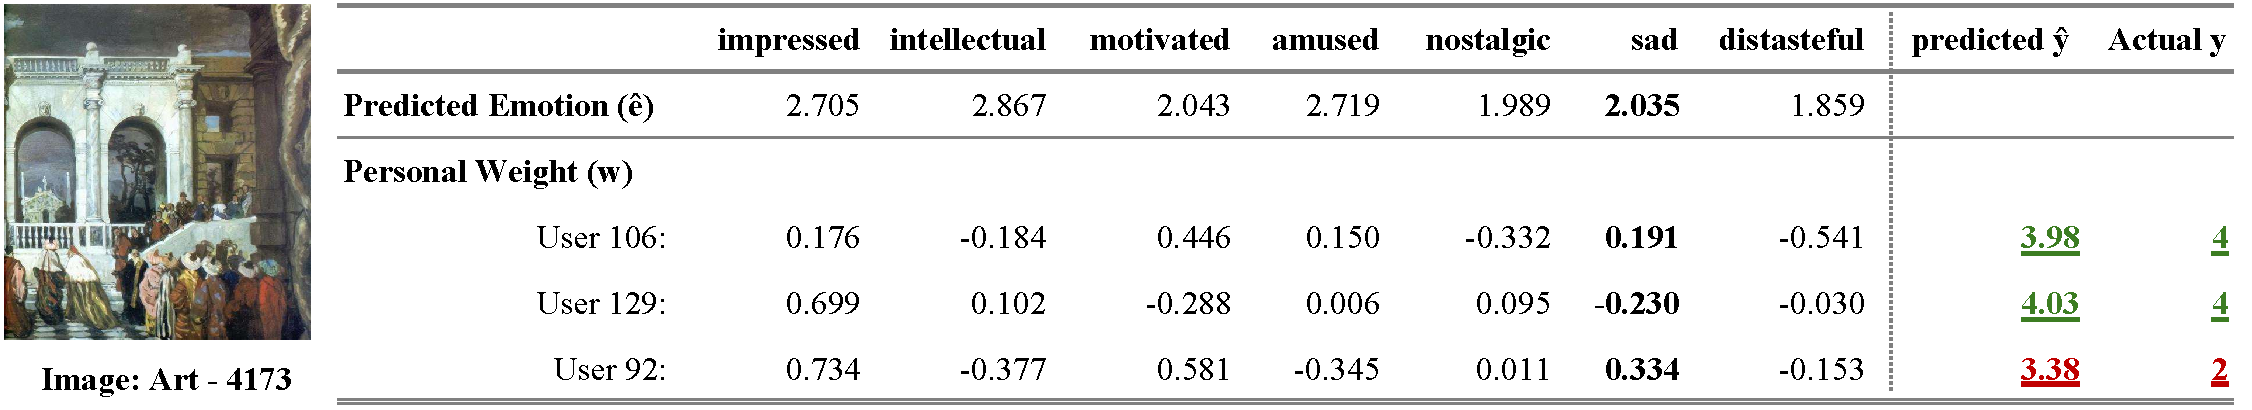
\includegraphics[width=\linewidth]{Table_Figure/fig_qualitative.pdf}
    \caption{\textbf{Qualitative personal-formula example and failure case.} 
    \item All three users rated the same artwork (image 4173). The first row shows the Stage-1 emotion vector on its 1--5 scale; these values are standardized before entering the personal head. The displayed coefficients are total
    emotion-space weights $\mathbf w_{\mathrm{tot}}$. The predictions are those of the complete anchored model, including the raw-feature population
    prediction and personal intercept. Users 106 and 129 have opposite-sign Sad
    weights ($w_{\mathrm{sad}}=+.191$ and $-.230$) and predictions within .03 of
    their recorded scores. User 92 has the largest error among the remaining users
    who rated the image ($y=2.0$, $\hat y=3.38$) and is shown as a failure case.}
    \label{fig:qualitative}
\end{figure*}


\section{Scope of the Evidence}

The seven personal coefficients describe how an individual's prediction
departs from a population branch fitted on raw visual features; they do not
decompose that shared branch. The computational diagnostics provide evidence
for owner, weight, and image specificity within the evaluated model. No
participant inspected or edited a formula in this study, so usability and
successful human correction remain questions for a user study. Comparisons with published ICI and MIR
numbers are descriptive only because their features and protocols differ; the
content-free Random control also reaches a similar range.

% --------------------------------------------
{
\small
\bibliographystyle{ieeenat_fullname}
\bibliography{main}
}
\end{document}